\section{Discussion}
\subsection{Agent diversity and quality are critical}
To investigate the role of agent diversity and quality in \texttt{TUMIX} performance, we compare groups of agents with varying levels of diversity and capability, as shown in Fig.~\ref{fig:diversity_quality_HLE_GPQA} and Appendix~Table~\ref{table: overall results TUMIX variants}. Under the same amount of refinement rounds and inferences, increasing the number of agents from 1 to 3 to 15 leads to substantial improvements in both coverage and average score across rounds on HLE and GPQA, indicating that diversity significantly benefits performance. Moreover, comparing a single strong agent with a single weak agent (see Appendix~Table~\ref{table: acc round evolution}, where \texttt{CS$_{\text{gs}}$} achieves higher first-round scores than \texttt{w/o TTS}), we observe that higher-quality agents consistently yield better coverage and higher average scores.

\textbf{Code Interpreter and Search increase answer diversity.}\quad In Fig.~\ref{fig:search_code_text}, we evaluate three settings where each agent group consists of three agents, each sampling five times per round. The groups differ in their tool access: in Code\_Text, agents cannot access Search; in Search\_Text, they cannot access the Code Interpreter; and in Code\_Search\_Text, agents have full access to both. While the average agent quality (as measured by first-round scores in Appendix~Table~\ref{table: acc round evolution}) is comparable across groups, the group with access to both Code Interpreter and Search achieves notably higher coverage and average scores. This result demonstrates that integrating complementary tools within agents enhances both reasoning and answer diversity, thereby facilitating more effective problem solving.

\begin{figure*}[ht]
  \centering
  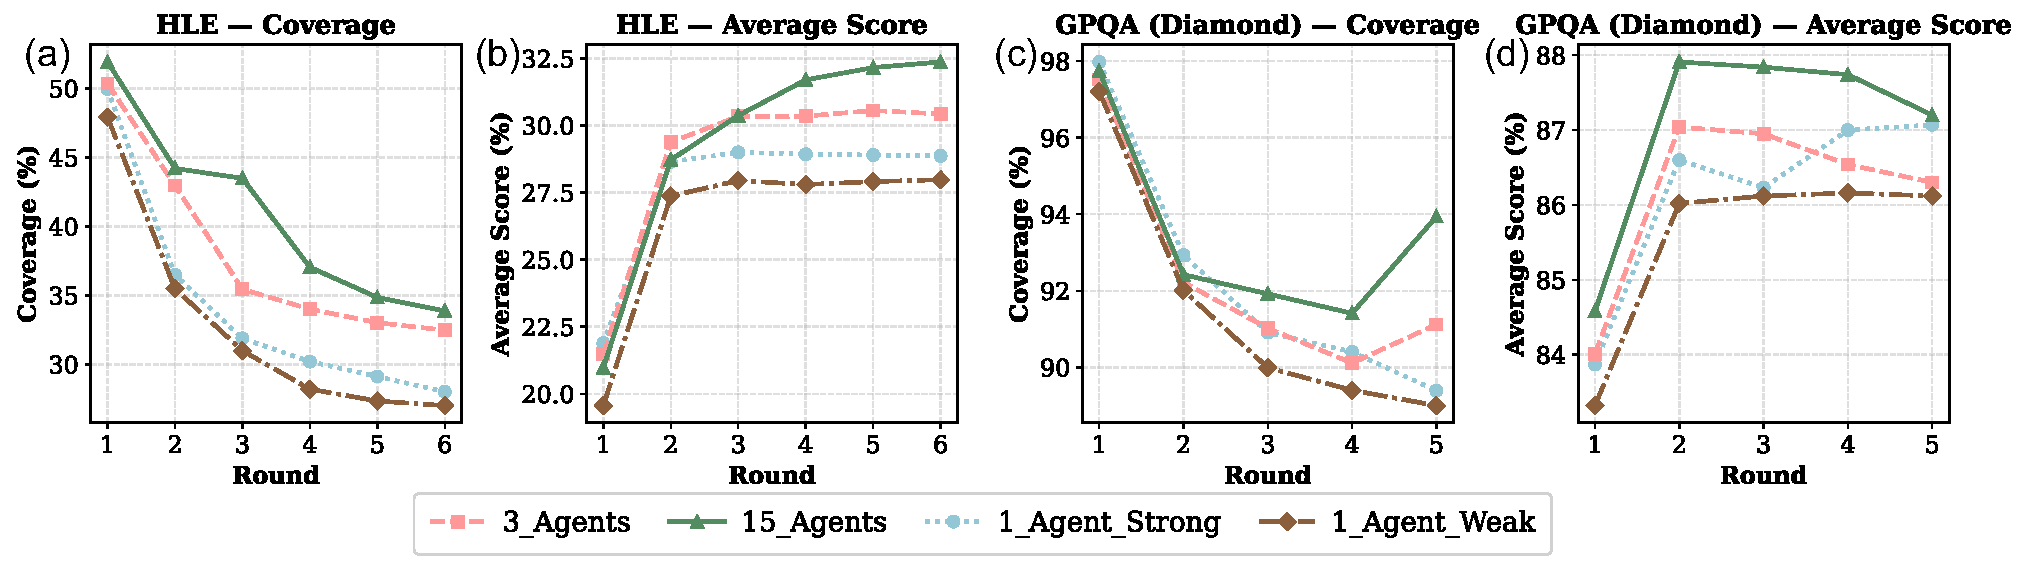
\includegraphics[width=0.98\linewidth]{Figures/diversity_quality_HLE_GPQA.pdf}
   \caption{Coverage and average score vs. rounds under varying agent diversity and quality. In 15\_Agents, all 15 varied pre-designed agents generate one answer each round. In 3\_Agents, three strong agents (\texttt{C$^+$}, \texttt{CS$_{\text{gs}}$}, and \texttt{CSG$_{\text{gs}}$}) each samples 5 times per round. In 1\_Agent\_Strong and 1\_Agent\_Weak, \texttt{CS$_{\text{gs}}$} and \texttt{w/o TTS} sample 15 times, respectively.}
   \label{fig:diversity_quality_HLE_GPQA}
\end{figure*}

\begin{figure}[ht]
    \centering
    % First figure
    \begin{minipage}[ht]{0.59\textwidth}
        \centering
        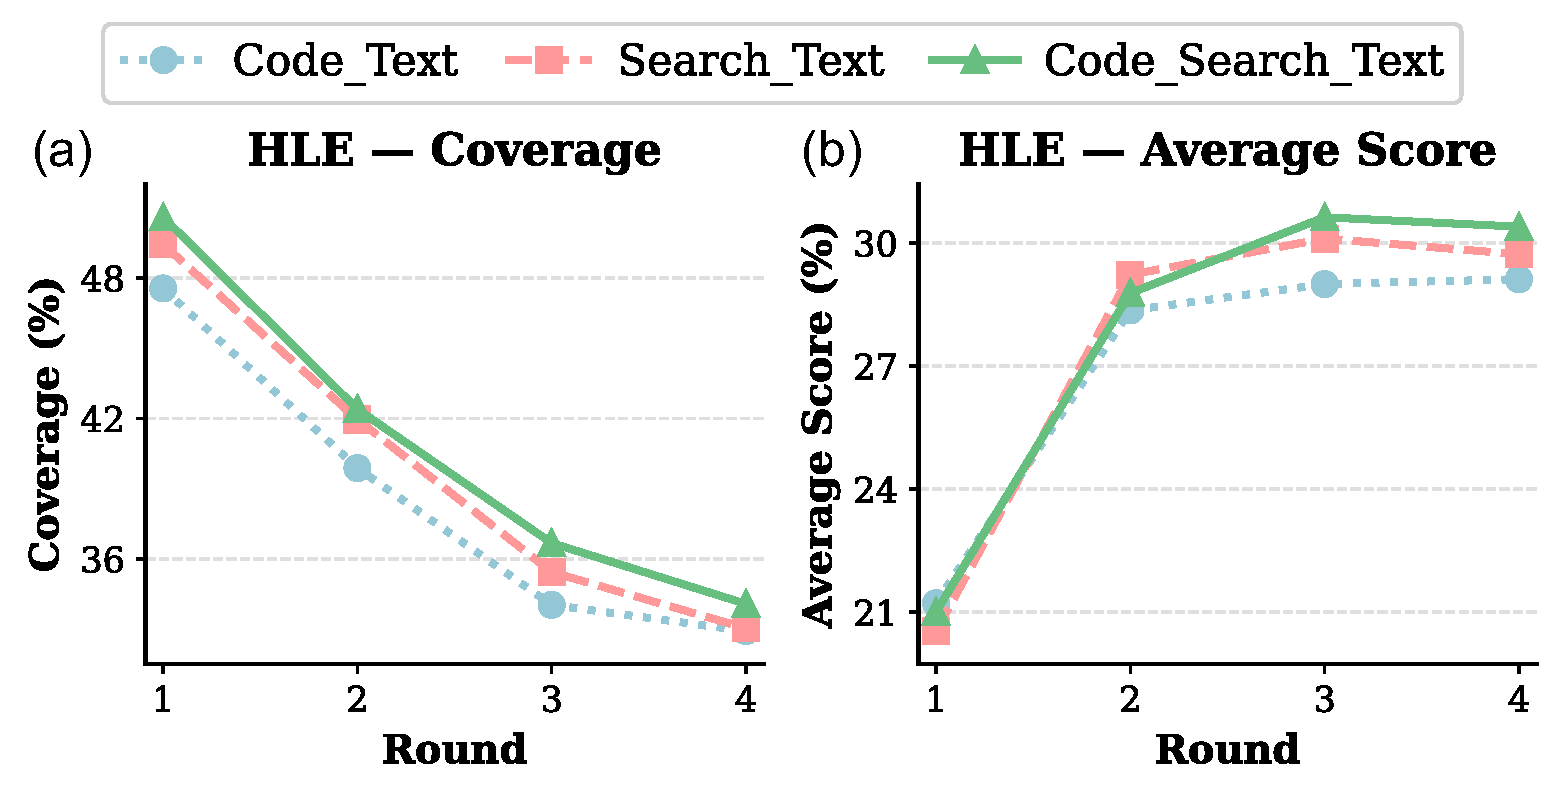
\includegraphics[width=0.98\linewidth]{Figures/search_code_text.pdf}
        \caption{Comparison of groups all with three agents but either partial or full accesses to textual reasoning, coding, and search: Code\_Text (\texttt{CoT}, \texttt{C}, \texttt{C$^+$}), Search\_Text (\texttt{CoT}, \texttt{S}, \texttt{CS$_{\text{gs}}$}), and Code\_Search\_Text (\texttt{CS$_{\text{gs}}$}, \texttt{C$^+$}, and \texttt{CSG$_{\text{gs}}$}).}
        \label{fig:search_code_text}
    \end{minipage}%
    \hfill
    % Second figure
    \begin{minipage}[ht]{0.39\textwidth}
        \centering
        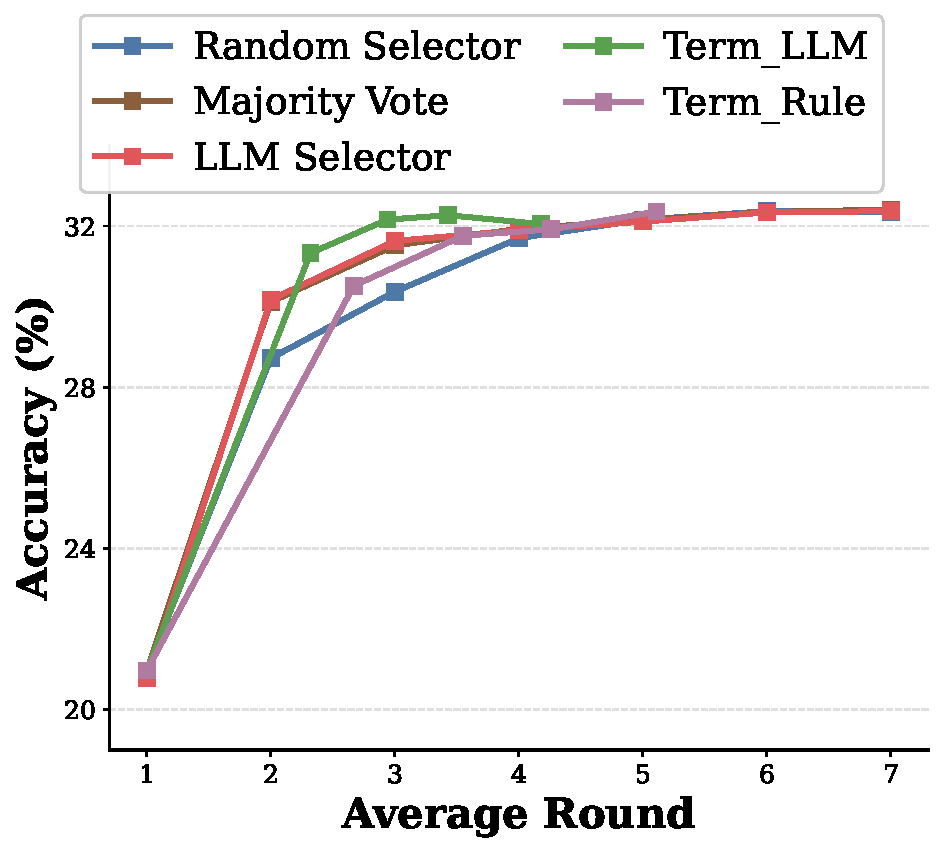
\includegraphics[width=0.98\linewidth]{Figures/selector_comparison.pdf}
        \caption{Comparison of refinement termination and answer selection strategies for higher accuracy with lower costs.}
        \label{fig:selector_comparison}
    \end{minipage}
\end{figure}

\subsection{Termination and selection methods}
\label{Sec: Experiments of Termination and selection methods}
\textbf{Achieving optimal performance at 49\% cost.}\quad Tasks of varying difficulty require different numbers of refinement rounds, and excessive refinement can even degrade accuracy (see Fig.~\ref{fig:acc_evolution_by_round}b). Thus, an effective termination strategy is essential to balance performance and cost. We evaluate two termination strategies (Sec.~\ref{subsection:Termination and selection}): 
1) \textbf{Term\_LLM}, which queries the LLM to decide when to stop refinement, subject to a minimum round constraint; and 
2) \textbf{Term\_Rule}, which stops once the majority answer stabilizes across two consecutive rounds, also with a minimum round constraint. We vary the minimum number of rounds to examine how performance evolves as the number of rounds increases in Fig.~\ref{fig:selector_comparison}, and we compare their peak performance in Appendix~Table~\ref{table: overall results TUMIX variants}. Term\_LLM achieves nearly the same peak accuracy as unlimited refinement, but with substantially fewer rounds. On average, Term\_LLM retains optimal performance while requiring only 49\% of the LLM inferences needed to obtain the final answer (LLM judging cost counted). The token costs are even less (approximately 46\%), as the number of inference tokens used in later rounds exceeds that of the first two rounds. This demonstrates the effectiveness of using LLM-as-Judge to determine when refinement is sufficient and answers can be finalized. However, Term\_LLM still requires a minimum number of refinement rounds (set to two across all benchmarks). This is because we observe that LLMs tend to be overconfident and may terminate refinement early, even when additional refinement could improve performance. For example, as shown in Fig.~\ref{fig:selector_comparison} green curve, setting the minimum refinement rounds to one leads to worse performance.

For answer selection, we compare three strategies: (1) randomly choosing one agent’s answer, (2) majority voting, and (3) LLM-based selection with LLM-as-Selector. Fig.~\ref{fig:selector_comparison} shows that majority voting and LLM-based selection consistently outperform random choice, especially in early rounds when agent answers diverge. However, once answers converge in later rounds, all selection methods yield similar results, and their impact becomes negligible. The multi-round refinement process is also a selection process. We also explore improved selection based on LLM token confidence~\citep{fu2025deep}, but observe no significant differences (Appendix~Fig.~\ref{fig:logprob_compare}).

\subsection{Human pre-designed agents vs. LLM generated agents}
\label{sec:Human pre-designed agents vs. LLM generated agents}
\begin{figure*}[ht]
  \centering
  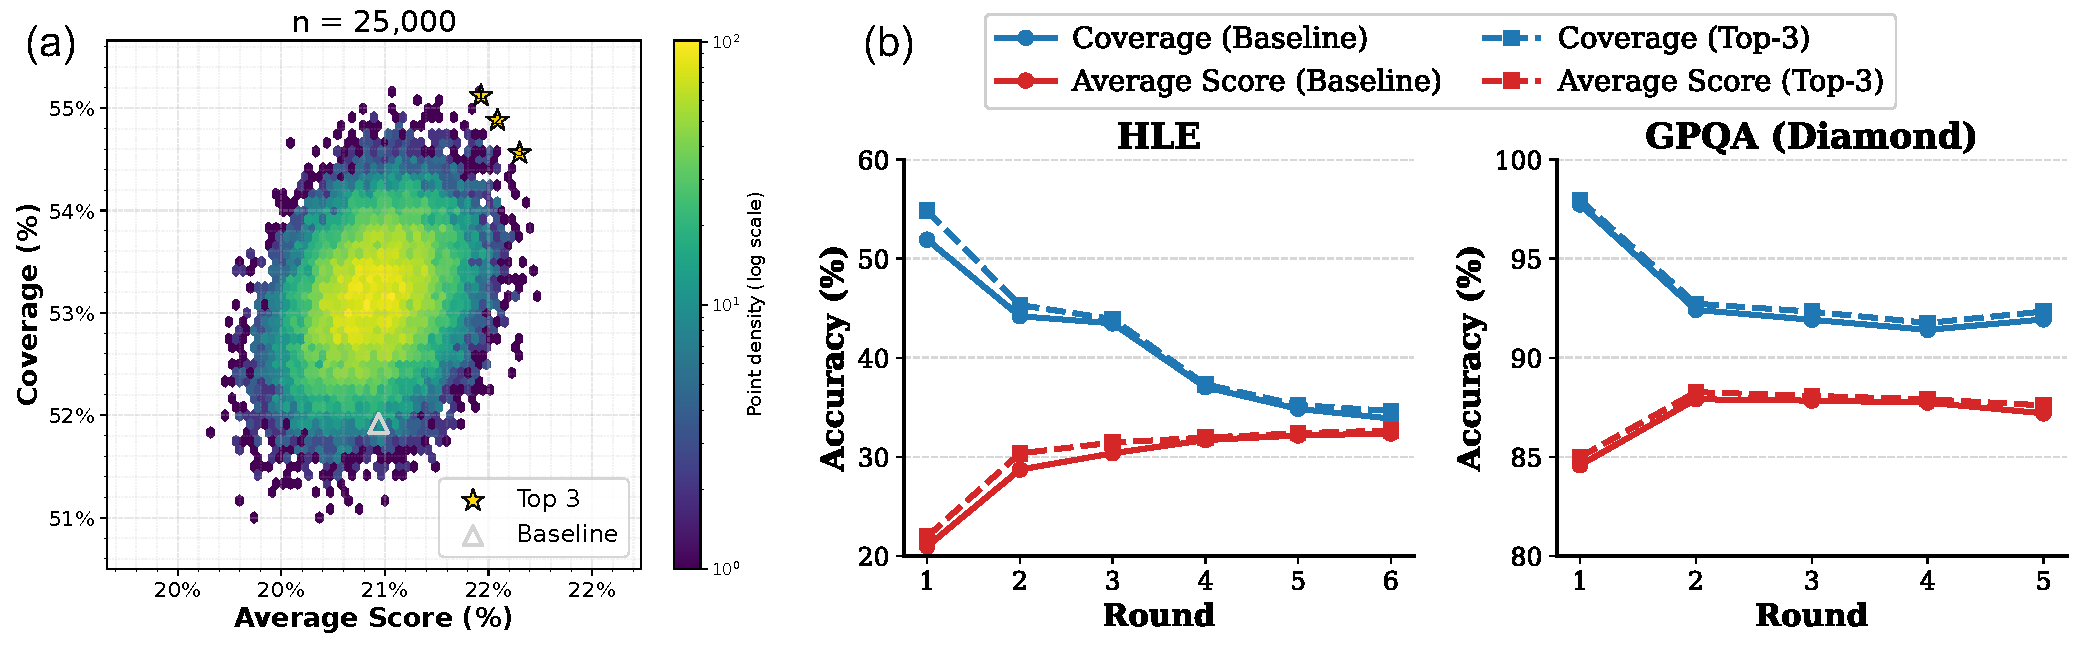
\includegraphics[width=0.95\linewidth]{Figures/LLM_generated_agents.pdf}
   \caption{We evaluate the coverage and average score of 25,000 15-agent combinations sampled from 30 agents (15 pre-designed and 15 LLM-generated). Baseline refers to the original 15 pre-designed agents. Top-3 refers to the three sampled combinations with the highest joint performance in coverage and average score.}
   \label{fig:LLM_generated_agents}
\end{figure*}

The human-designed agents and their tool-use strategies are built on existing frameworks or intuition. To explore whether stronger agents can be discovered automatically, we query Gemini-2.5-Pro with current agent code examples and ask it to generate full implementations of more diverse and high-quality ones, where the agent prompts and frameworks are all determined by LLMs. This yield 25 diverse agents beyond the 15 human-designed ones. From these, we retain the 15 that perform best in HLE with first-round answer generation. We then combine the 15 human-designed and 15 LLM-generated agents into a pool of 30, randomly sample groups of 15, and evaluate their average score and coverage (Fig.~\ref{fig:LLM_generated_agents}a). Compared to the baseline of 15 human-designed agents (gray triangle), many mixed groups achieve both higher average score and coverage. We select the top-3 groups based on the combined metric
\begin{equation}
\label{eq:combined_score}
\text{Combined Score}_i \;=\; 
\frac{\text{Coverage}_i}{\mathbb{E}\!\left[\text{Coverage}\right]} 
\;+\; 
\frac{\text{Average Score}_i}{\mathbb{E}\!\left[\text{Average Score}\right]}.
\end{equation}

As shown in Fig.~\ref{fig:LLM_generated_agents}b, these groups outperform the original \texttt{TUMIX} in both HLE and GPQA. This demonstrates that increasing agent diversity and quality improves effectiveness, and that LLM-generated agents hold strong potential for further enhancing \texttt{TUMIX}. Appendix~Table~\ref{tab:baseline_agents} describes each generated agent, whose strategies differ substantially from the original ones beyond prompt variations. Appendix~Table~\ref{tab:agent_group_original_top3} presents the agents in each top-3 group, with roughly half overlapping with the original group.

\textbf{Evolve agents in each round to enhance the diversity}\quad In all previous experiments, the agent set remained fixed across refinement rounds. We now investigate whether dynamically varying agent types per round can improve performance. As shown in Appendix Table~\ref{table: overall results TUMIX variants}, the variant \texttt{TUMIX-EvolveD}, which randomly selects agents from the top-3 sets each round, performs slightly worse than the fixed variant \texttt{TUMIX-Evolve} across all three benchmarks.

\textbf{Impact of number of agent types}\quad 
We next examine the marginal benefit of increasing the number of agents in \texttt{TUMIX}. Agents are randomly sampled from the pool of 30, with each contributing one inference per round. To isolate this effect, we exclude termination and selection and report the evolution of peak average accuracy across rounds. As shown in Fig.~\ref{fig:peak_accuracy_vs_agents}, accuracy rises quickly when the number of agents is below 12, but gains become negligible thereafter. This indicates that beyond a certain point, increasing agent types and inference budget yields little benefit, as additional candidate answers make round-by-round selection more challenging. Based on these results, we decide to only include 15 agents in \texttt{TUMIX} to balance performance and cost.

\subsection{Scaling Curves: Performance vs. Costs}

\begin{comment}
\begin{figure*}[ht]
  \centering
  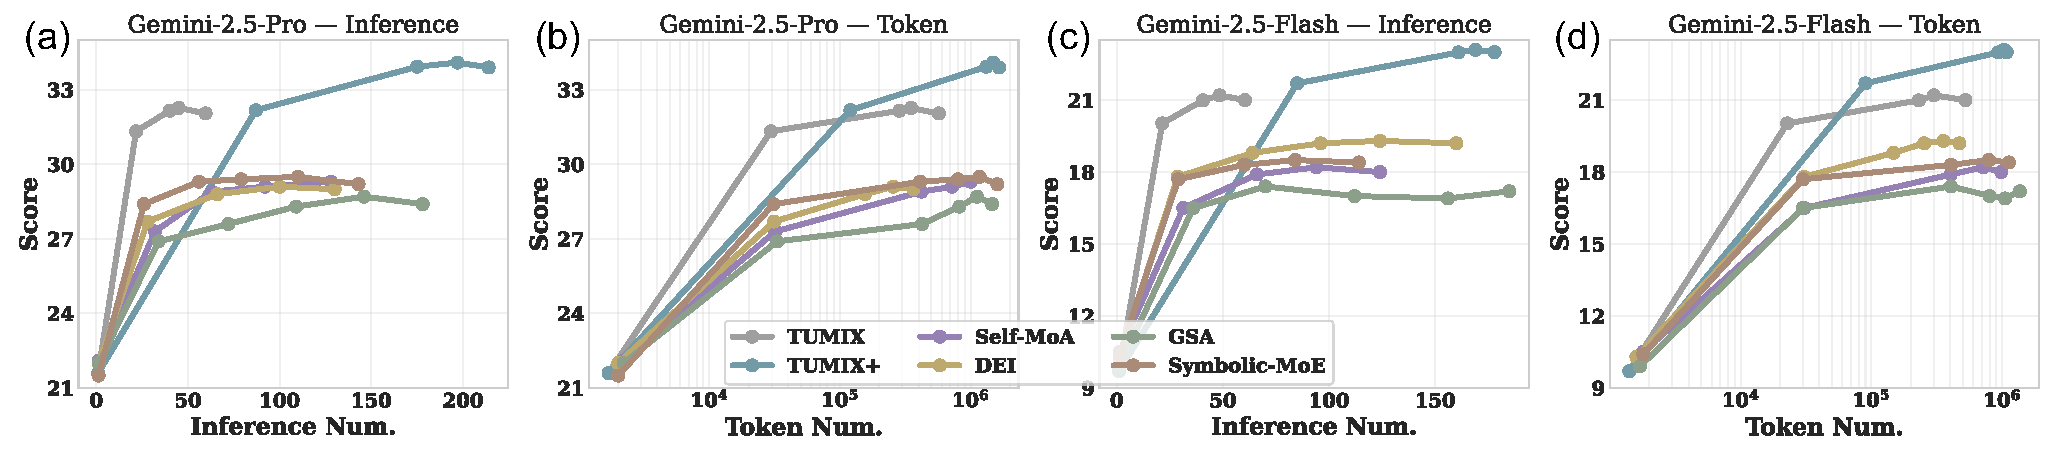
\includegraphics[width=0.98 \linewidth]{Figures/Scaling_law.pdf}
   \caption{Scaling behavior of HLE scores relative to inference cost and total token count across different tool-augmented test-time scaling methods, where the token count includes both input and output tokens.}
   \label{fig:Scaling_law}
\end{figure*}
\end{comment}

\begin{figure}[ht]
    \centering
    % First figure
    \begin{minipage}[ht]{0.59\textwidth}
        \centering
        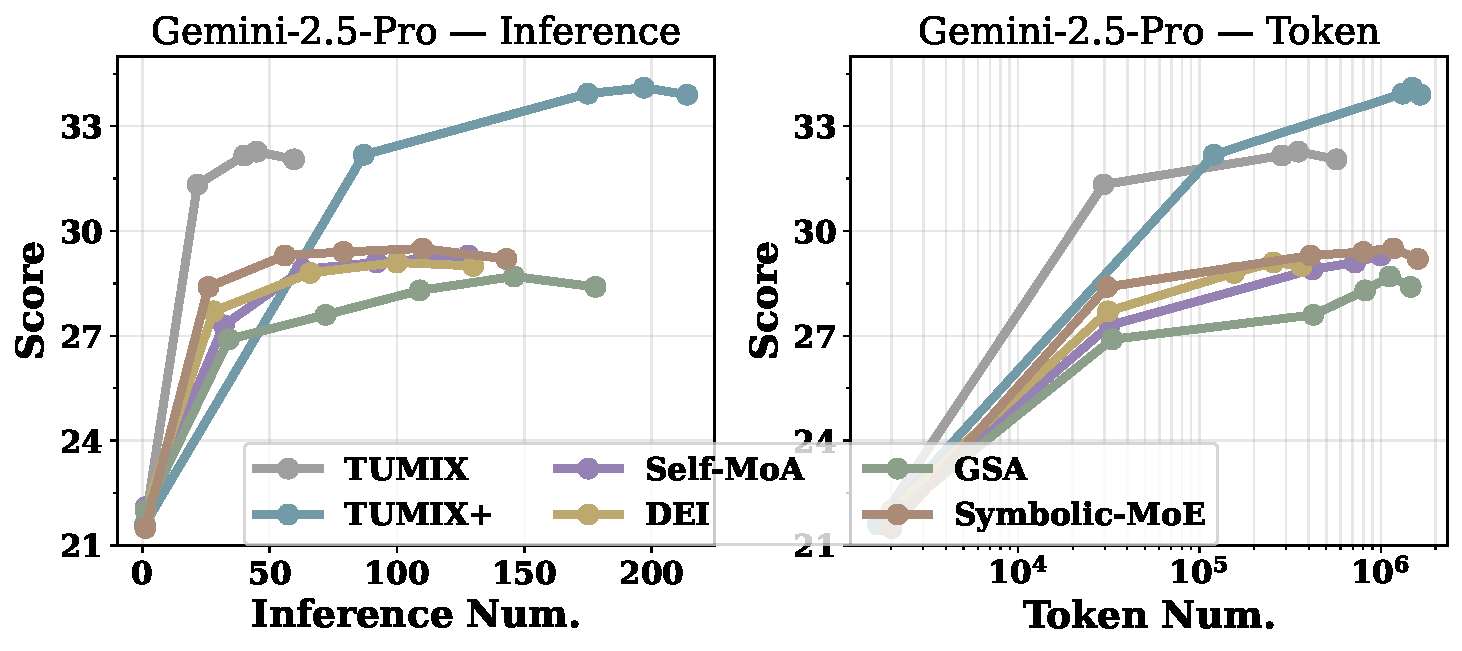
\includegraphics[width=0.98\linewidth]{Figures/scaling_pro_only.pdf}
        \caption{Scaling behavior of HLE scores relative to inference cost and total token count across different tool-augmented test-time scaling methods, where the token count includes both input and output tokens.}
        \label{fig:Scaling_law}
    \end{minipage}%
    \hfill
    % Second figure
    \begin{minipage}[ht]{0.39\textwidth}
        \centering
        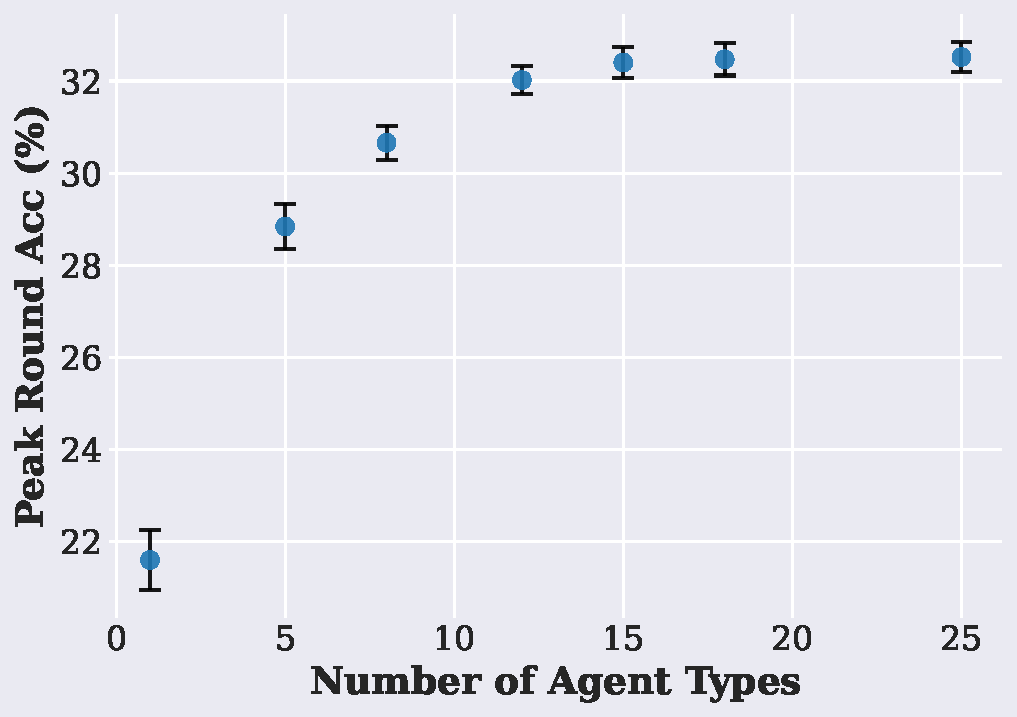
\includegraphics[width=0.92\linewidth]{Figures/peak_accuracy_vs_agents.pdf}
        \caption{Peak round accuracy versus number of agent types. Agent types randomly sampled from the 30 well-performing agents with three repetition. Each agent infers once per round.}
        \label{fig:peak_accuracy_vs_agents}
    \end{minipage}
\end{figure}

We compare the scaling behavior of different tool-augmented test-time scaling methods in terms of inference and token costs. In \texttt{TUMIX} and \texttt{Self-MoA}, scaling comes from adding more refinement rounds; in \texttt{GSA}, \texttt{DEI}, and \texttt{Symbolic-MoE}, from repeating inference; and in \texttt{TUMIX+}, from both. As shown in Fig.~\ref{fig:Scaling_law} and Appendix~Fig.~\ref{fig:Scaling behavior of Gemini-2.5-flash}, \texttt{TUMIX} consistently outperforms other methods, achieving the highest scores with fewer inference steps and tokens. \texttt{TUMIX+} pushes peak performance further by repeating inference four times across the first two refinement rounds, but at substantially higher cost and lower efficiency. Overall, test-time scaling demands far more inferences and roughly two orders of magnitude more tokens, a seemingly unavoidable trade-off.